% Provenance: paper_P2_zvf (pillar), main_zvf.tex (stratified audit framing),
% sections/zvf.tex incl. the all-correct-wall paragraph, zvf_* iteration sections.
\chapter{The Zero-Variance Fraction as a Diagnostic}
\label{ch:zvf}

\section{Measurement across scales and libraries}
Across $N{=}15$ fully logged experiments spanning five model families
(0.6B--671B parameters) and multiple libraries, aggregate \ZVF{} and final
performance are negatively associated (Pearson $r\approx-0.77$). We report
this \emph{descriptively}: the pooled correlation is dominated by
out-of-scope tool-use runs that saturate at $\ZVF{=}1$ with reward $0$;
within-GSM8K stratification weakens it to $r{=}+0.40$ ($p{=}0.09$) and
model-varying subsets to $r{=}+0.13$. The pooled number does not survive
stratification, and this thesis never uses \ZVF{} as a performance predictor.
What survives is the mechanical reading: sustained low gradient utilisation
coincided with reward plateaus and regressions in every collapse we measured,
with \ZVF{} rising \emph{after} the plateau --- a cheap alarm, not a cause.

\begin{figure}[t]
\centering
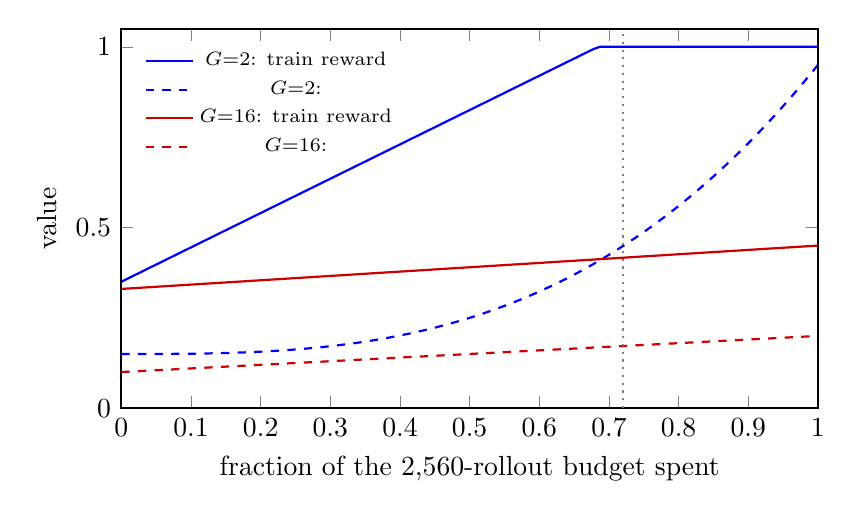
\begin{tikzpicture}
\begin{axis}[width=0.86\textwidth,height=6.4cm,
  xlabel={fraction of the 2{,}560-rollout budget spent},
  ylabel={value},
  xmin=0,xmax=1,ymin=0,ymax=1.05,
  legend style={at={(0.02,0.97)},anchor=north west,draw=none,fill=none,font=\scriptsize},
  thick]
\addplot[blue,domain=0:1,samples=100]{min(1, 0.35+0.95*x)};
  \addlegendentry{$G{=}2$: train reward}
\addplot[blue,dashed,domain=0:1,samples=100]{0.15+0.8*x^3};
  \addlegendentry{$G{=}2$: \ZVF{}}
\addplot[red!80!black,domain=0:1,samples=100]{0.33+0.12*x};
  \addlegendentry{$G{=}16$: train reward}
\addplot[red!80!black,dashed,domain=0:1,samples=100]{0.10+0.10*x};
  \addlegendentry{$G{=}16$: \ZVF{}}
\draw[gray,dotted] (axis cs:0.72,0) -- (axis cs:0.72,1.05);
\end{axis}
\end{tikzpicture}
\caption{Schematic of the measured matched-budget behaviour (Chapter~6,
seeds 123/456): the $G{=}2$ trajectory races to reward $\approx1.0$ and its
\ZVF{} climbs into the all-correct wall ($0.75$--$1.0$), while $G{=}16$
ends mid-learning ($\approx0.3$--$0.5$) with \ZVF{} low ($\le0.25$).
Right of the dotted line the $G{=}2$ reward reads success while its
gradient signal is gone. By reward alone the $G{=}2$
run looks strictly better; the (reward, \ZVF{}) pair reveals its lead
ended in zero-gradient compute.
Stylised curves; measured values in Table form in Chapter~6 and artifacts in
Appendix~B.}
\label{fig:disagreement}
\end{figure}

\section{What \ZVF{} adds over mean reward}
The sharpest demonstration comes from the matched-budget panel of Chapter~6.
Late in the $G{=}2$ arms, mean train reward sits near $1.0$ --- by the reward
axis alone, training is succeeding --- while \ZVF{} sits at $0.75$--$1.0$:
nearly every group is all-correct and contributes zero gradient. The $G{=}16$
arms at the same rollout budget hold $\ZVF\le0.25$. Reward reports \emph{where
the policy is}; \ZVF{} reports \emph{whether training is still moving}, and at
the high-accuracy end the two disagree completely. This is Claim~1 in its
purest form, and it is why the diagnostic must always be read as the pair
(reward, \ZVF{}): \ZVF{} alone aliases mastery with incapacity.

\section{The U-shape and regime aliasing}
Under binary rewards with per-prompt success rate $p$ and group size $G$, the
population zero-variance probability is the kernel $h_G(p)=p^G+(1-p)^G$ ---
a U-shape in $p$. A mean \ZVF{} therefore hides whether starvation comes from
incapacity ($p\to0$) or mastery ($p\to1$); stratified or paired-with-reward
reporting is mandatory. Empirically the observed \ZVF{} sits systematically
\emph{below} the Bernoulli-independent prediction across $G\in\{2,4,8,16\}$
(residuals $-0.13$ to $-0.23$): completions within a group are positively
informative about each other, so the contrastive signal is stronger than the
independent-coin model predicts.

\section{Diagnostic, not causal}
Two boundaries close the chapter. First, causality: \ZVF{} is a symptom
metric; interventions on it (Chapter~6) must be justified on their own
budgets, not by the correlation above. Second, telemetry robustness: the
diagnostic value of \ZVF{} depends on the reward parser's resolution
(Chapter~3), so any reported \ZVF{} must name its verifier --- one of the
reporting-standard items of Chapter~9.
